\documentclass{beamer} 


%\usetheme[height=7mm]{Rochester}
%\useinnertheme{rectangles}
%\useoutertheme{shadow}
%\setbeamertemplate{footline}{}
%\usecolortheme{orchid}
%\usecolortheme{whale}
\usecolortheme[RGB={0,70,6}]{structure} 

\definecolor{thegreen}{RGB}{0,80,6}

%\usefonttheme{serif}
\beamertemplatenavigationsymbolsempty
%\setbeamertemplate{items}[default] 
\setbeamertemplate{itemize item}{\small\bf\raise0.8pt\hbox{\guillemotright}} 
\setbeamertemplate{itemize subitem}{\small\bf\raise0.8pt\hbox{\guilsinglright}} 

\usepackage[T1]{fontenc}

\usepackage{graphicx,amsmath,unit,short,booktabs,tikz,pgfplots}
\graphicspath{{../fig/}}


\title{QGP parameter extraction via a global analysis of event-by-event flow coefficient distributions}

\author{
  Jonah E.\ Bernhard\inst{1}
  \and
  Christopher E.\ Coleman-Smith\inst{1} \\
  \and
  Peter W.\ Marcy\inst{2}
  \and
  Steffen A.\ Bass\inst{1}
}

\institute{
  \inst{1}Department of Physics \\ Duke University
  \and
  \inst{2}Department of Statistics \\ University of Wyoming
}
\date{20 July 2013}


\begin{document}



\frame[plain]{\titlepage}




\begin{frame}{Model to data comparison}
  \begin{onlyenv}<1>
    \centering
    \begin{tikzpicture}[node distance=2cm,semithick]
      %\draw[thick,->] (0,10) node[draw,rectangle,above] {Input parameters} -- ++(0,-1);
      \node (input) [rectangle,draw,align=center] {\textbf{\color{thegreen} Input parameters} \\ $\eta/s$, \ldots};
      \node (model) [below of=input,rectangle,draw,align=center] {\textbf{\color{thegreen} Model} \\ initial conditions, hydro, \\ sampler, UrQMD};
      \node (output) [below of=model,rectangle,draw,align=center] {\textbf{\color{thegreen} Output (observables)} \\ flows, spectra, \ldots};
      \draw[->] (input) -- (model);
      \draw[->] (model) -- (output);

      \node (data) [right of=output,node distance=6.1cm,rectangle,draw,align=center] {
        \textbf{\color{thegreen}Experimental data} \\[1ex]
        %\tikz\node [anchor=north west] {\includegraphics[width=3cm]{atlas-flows}};
        %\tikz\node [anchor=south west] {\includegraphics[width=3cm]{atlas-flows}};
        %\tikz\node at (0,0) {\includegraphics[width=3cm]{atlas-0}};
        %\vspace{2cm}\hspace{-.5cm}
        \includegraphics[width=3cm]{atlas-phi}
        \hspace{-.5cm}\vspace{-1cm}
        \includegraphics[width=3cm]{atlas-flows} \\[1cm]
        \includegraphics[width=3cm]{atlas-mult}
      };

      \draw[very thick,dashed,<->] (output) -- node[above] {\bf ?} (data); 
    \end{tikzpicture}
  \end{onlyenv}

  \begin{onlyenv}<2>
  The generic recipe:
  \begin{itemize}
    \item Choose a set of input parameters.
    \item Vary parameters, calculate observables.
    \item Determine parameters that optimally describe reality.
  \end{itemize}

  \sms

  Easy if the model is fast:
  \begin{itemize}
    \item Use e.g.\ MCMC to find the optimal parameters.
    \item Requires many points in parameter space, $\mathcal O(10^6)$ or more.
    \item Only feasible if the model runs in $\mathcal O(1 \ut{second})$.
  \end{itemize}

  \sms

  Heavy-ion collision models are {\em not} ``fast''.
  \begin{itemize}
    \item Need a different approach.
  \end{itemize}
  \end{onlyenv}
\end{frame}



\begin{frame}{Slow models}
  Strategy:  emulate the model.

  \begin{itemize}
    \item Run at predetermined set of parameter points.
      \begin{itemize}
        \item Latin-hypercube sample.
      \end{itemize}

    \item Interpolate between points.
      \begin{itemize}
        \item Emulator.
      \end{itemize}
  \end{itemize}
\end{frame}



\begin{frame}{Latin-hypercube sampling}
  \begin{itemize}
    \item Provides an optimal set of parameter points.
    \item \emph{Maximizes} the \emph{minimum} distance between points.
  \end{itemize}

  \centering
  \includegraphics<1>{lhs1}
  \includegraphics<2>{lhs2}
\end{frame}




\begin{frame}{Gaussian processes}

  \begin{itemize}
    \item \emph{Assume} the model is a Gaussian process.
    \item A Gaussian \emph{process} is a generalization of a Gaussian \emph{distribution}.
      \begin{itemize}
        \item Draw a set of Gaussian values with a specified covariance.
      \end{itemize}
  \end{itemize}

  \sms

  \begin{columns}[c]
    \column{.5\textwidth}
      \begin{equation*}
        \text{cov}(x_1,x_2) \propto \exp \biggl[ -\frac{(x_1 - x_2)^2}{2\ell^2} \biggr]
      \end{equation*}
    \column{.5\textwidth}
    \includegraphics[width=\textwidth]{gpr1}
  \end{columns}

  \flushright\tiny \emph{Gaussian Processes for Machine Learning}, Rasmussen and Williams, 2006.
\end{frame}




\begin{frame}{Gaussian process emulators}

  \begin{itemize}
    \item Prior:  the model is a Gaussian process.
    \item Posterior:  Gaussian process conditioned on model outputs.
  \end{itemize}

  %\sms

  \begin{tikzpicture}
    \draw[very thick,->] (0,0) node[left,align=center] {\ \ prior \\ \includegraphics[width=.28\textwidth]{gpr1}} -- 
    node[above] {linear algebra} (2.5,0) node[right,align=center] {\ \ \ \ posterior \\ \includegraphics[width=.45\textwidth]{gpr2}};
  \end{tikzpicture}
  
  %\sms

  \begin{itemize}
    \item Emulator is a fast surrogate to the actual model.
    %\item Provides a Gaussian at all points in parameter space.
      \begin{itemize}
        %\item Narrower (more certain) near calculated points.
        %\item Wider (less certain) in gaps.
        \item More certain near calculated points.
        \item Less certain in gaps.
      \end{itemize}
  \end{itemize}
\end{frame}





\begin{frame}{The data}
  \begin{itemize}
    \item ATLAS event-by-event flow distributions $v_n$, $n = 2$--6.
    \item Could provide a much more sensitive probe than average flows
      \begin{itemize}
        \item especially high-order ($n > 3$).
      \end{itemize}
  \end{itemize}

  \mds

  \centering
  \includegraphics[width=\textwidth]{atlas-flows}
  \flushright{\tiny hep-ex/1305.2942}
\end{frame}


\begin{frame}{Data reduction}
    \begin{itemize}
      \item Fit to ``Generalized Reverse Weibull'' distribution.
        \begin{itemize}
          \item Represent each distribution by four fit parameters.
        \end{itemize}
    \end{itemize}

    \vspace{-.5cm}
    \begin{equation*}
      f(x;m,s,\alpha,\gamma) = \frac{\alpha}{s\,\Gamma(\gamma)} \biggl( \frac{x-m}{s} \biggr)^{\alpha\gamma-1} \exp \biggl[ -\biggl( \frac{x-m}{s} \biggr)^\alpha \biggr]
    \end{equation*}

    \centering
    \includegraphics<1>[width=\textwidth]{grw2}
    \includegraphics<2>[width=\textwidth]{grw3}

\end{frame}


\begin{frame}{The model}
  Modern version of the OSU+Duke hybrid model VISHNU (Viscous Hydro and UrQMD):
  \begin{itemize}
    \item MC-Glauber/KLN initial conditions
    \item 2+1 viscous hydro (OSU)
    \item Cooper-Frye hypersurface sampler (OSU)
    \item UrQMD
  \end{itemize}
  Similar to OSU iEBE, but organized differently; different analysis.
\end{frame}


\frame{\centering\textbf{Main goal} \\ \mds Calibrate the event-by-event model to ATLAS flow distributions.}


\begin{frame}{Experiment design}
  \begin{itemize}
    \item 256 Latin-hypercube points across 5 parameters:
      \begin{itemize}
        \item IC normalization
        \item IC-specific parameter (wounded nucleon / binary collision for Glauber, saturation exponent for KLN)
        \item hydro start time $\tau_0$
        \item viscosity $\eta/s$
        \item shear stress relaxation time $\tau_\Pi$
      \end{itemize}
    \item Observables:
      \begin{itemize}
        \item $v_n$ distributions
        \item multiplicities
        \item identified particle spectra
        \item \ldots
      \end{itemize}
  \end{itemize}
\end{frame}





\begin{frame}{CPU time}
  \begin{itemize}
    \item 3 centrality bins
    \item 256 points/bin
    \item 1000 events/point
    \item $\sim 1$ hour/event
  \end{itemize}
  \mds
  \centering $\sim 768\,000 \ut{CPU hours} \sim 87 \ut{years}$
  \mds
  \begin{itemize}
    \item Open Science Grid (OSG)
  \end{itemize}
\end{frame}



\begin{frame}{EbE-OSG:  job automation}
  \centering

  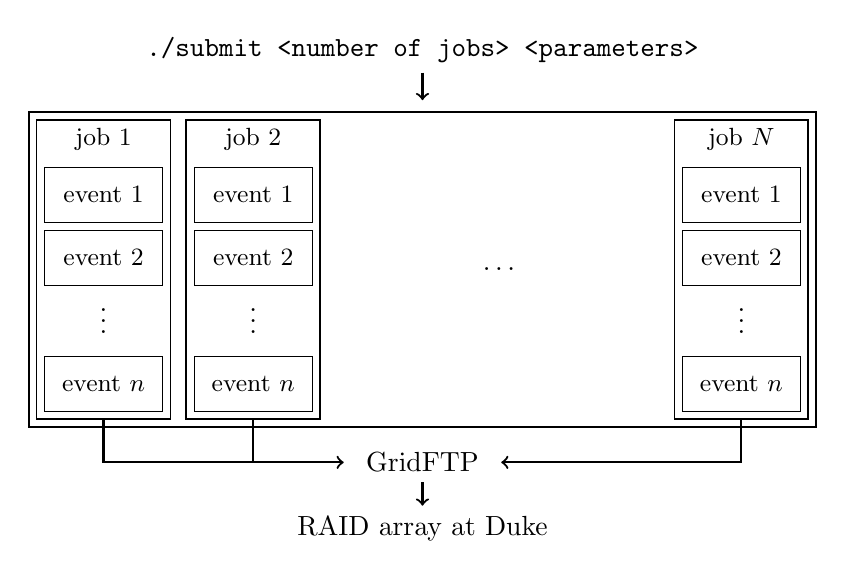
\begin{tikzpicture}
    \draw[thick,->] (0,2.5) node[above] {\tt ./submit <number of jobs> <parameters>} -- (0,2.15);

    \draw[thick] (-5,-2) rectangle (5,2);

    \draw[semithick] (-4.9,-1.9) rectangle (-3.2,1.9);
    \node at (-4.05,1.65) {\small job 1};
    \node at (-4.05,-.55) {\vdots};
    \draw (-4.8,0.6) rectangle node {\small event 1} (-3.3,1.3);
    \draw (-4.8,-.2) rectangle node {\small event 2} (-3.3,.5);
    \draw (-4.8,-1.8) rectangle node {\small event $n$} (-3.3,-1.1);

    \draw[semithick] (-3.0,-1.9) rectangle (-1.3,1.9);
    \node at (-2.15,1.65) {\small job 2};
    \node at (-2.15,-.55) {\vdots};
    \draw (-2.9,0.6) rectangle node {\small event 1} (-1.4,1.3);
    \draw (-2.9,-.2) rectangle node {\small event 2} (-1.4,.5);
    \draw (-2.9,-1.8) rectangle node {\small event $n$} (-1.4,-1.1);

    \node at (1,0) {\ldots};

    \draw[semithick] (3.2,-1.9) rectangle (4.9,1.9);
    \node at (4.05,1.65) {\small job $N$};
    \node at (4.05,-.55) {\vdots};
    \draw (3.3,0.6) rectangle node {\small event 1} (4.8,1.3);
    \draw (3.3,-.2) rectangle node {\small event 2} (4.8,.5);
    \draw (3.3,-1.8) rectangle node {\small event $n$} (4.8,-1.1);

    \draw[thick,->] (0,-2.7) node[above] {GridFTP} -- (0,-3) node[below] {RAID array at Duke};
    \draw[thick,->] (-4.05,-1.9) -- (-4.05,-2.45) -- (-1,-2.45);
    \draw[thick,->] (4.05,-1.9) -- (4.05,-2.45) -- (1,-2.45);
    \draw[thick] (-2.15,-1.9) -- (-2.15,-2.45);

  \end{tikzpicture}

  \flushright \footnotesize \url{github.com/jbernhard/ebe-osg}
\end{frame}



\begin{frame}
  \includegraphics[width=\textwidth]{user_hours_last_week}
  \begin{itemize}
    \item roughly $500\,000$ events complete
  \end{itemize}
\end{frame}


\begin{frame}{EbE analysis}
  \begin{itemize}
    \item Python + Numpy/Scipy
    \item parses event files
    \item calculates flows \& fits flow distributions
    \item calculates other observables
    \item makes common plots (Matplotlib)
  \end{itemize}

  \mds
  Planned:
  \begin{itemize}
    \item store results in database via ORM
    \item optimization via custom C++ extentions
  \end{itemize}

  \bgs
  \flushright \footnotesize \url{github.com/jbernhard/ebe-analysis}
\end{frame}


\begin{frame}
  \centering
  \textbf{Preliminary results} \\ 
  \bgs
  \emph{analysis of uncalibrated Latin-hypercube sample point} \\
  \bgs 
  two centrality bins, 0--5\% and 20--25\% \\
  1000 events each \\
  \bgs
  MC-Glauber with $\alpha = 0.06$
  \begin{equation*}
    \eta/s = 0.29
    \qquad
    \tau_0 = 0.93 \ut{fm}
  \end{equation*}
\end{frame}


\begin{frame}{$v_2$ distributions}
  \centering
  \includegraphics{v2}
\end{frame}


\begin{frame}{$v_3$ distributions}
  \centering
  \includegraphics{v3}
\end{frame}


\begin{frame}{Identified particle spectra}
  \centering
  \includegraphics{pT}
\end{frame}


\begin{frame}{Multiplicity}
  \centering
  \includegraphics{mult} \\[-.4cm]
  \includegraphics[height=3cm]{atlas-mult-20-25}
  \hspace{2cm}
  \includegraphics[height=3cm]{atlas-mult-0-5}
\end{frame}


\begin{frame}{Goals}
  \begin{itemize}
    \item Higher-order flows $v_4,v_5,v_6$.
    \item More realistic model (IP-Glasma, 3+1D, \ldots).
    \item Systematically analyze all events.
    \item Train emulator to calculated flow distributions, identified particles, etc.
    \item Calibrate parameters to data.
      \begin{itemize}
        \item Which are the most important?
      \end{itemize}
    \item Improve statistics for likely parameters.
  \end{itemize}
\end{frame}







\end{document}
